\documentclass[12pt]{article}
 \usepackage[margin=1in]{geometry} 
\usepackage{amsmath,amsthm,amssymb,amsfonts}
\usepackage{graphicx}
\usepackage{array}
\newcolumntype{P}[1]{>{\centering\arraybackslash}p{#1}}
\newcommand{\N}{\mathbb{N}}
\newcommand{\Z}{\mathbb{Z}}
 
\newenvironment{problem}[2][Problem]{\begin{trivlist}
\item[\hskip \labelsep {\bfseries #1}\hskip \labelsep {\bfseries #2.}]}{\end{trivlist}}
%If you want to title your bold things something different just make another thing exactly like this but replace "problem" with the name of the thing you want, like theorem or lemma or whatever
 
\begin{document}
 
%\renewcommand{\qedsymbol}{\filledbox}
%Good resources for looking up how to do stuff:
%Binary operators: http://www.access2science.com/latex/Binary.html
%General help: http://en.wikibooks.org/wiki/LaTeX/Mathematics
%Or just google stuff
 
\title{Homework-2 \\ Feature Descriptors,Homographies and RANSAC}
\author{N Dinesh Reddy \\ dnarapur@andrew.cmu.edu }

\newpage

\maketitle
\section{keypoint Detector}

\begin{problem}{1.1}
Code described in CreateGaussianPyramid.m\\
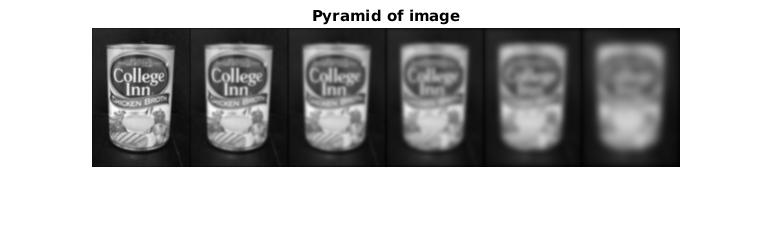
\includegraphics[scale = 0.4]{results/Gaupyr} 
\end{problem}
\begin{problem}{1.2}
Code described in CreateDoGPyramid.m \\
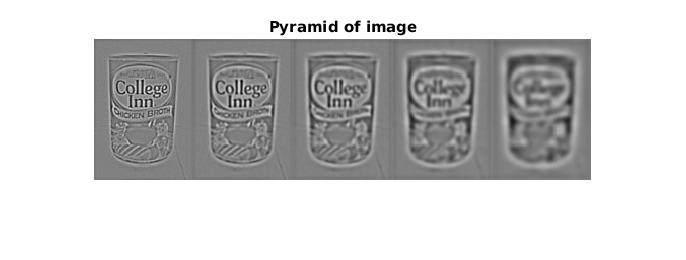
\includegraphics[scale = 0.4]{results/DoGpyr} 
\end{problem}
\begin{problem}{1.3}
Code described in computePrincipalCurvature.m 
\end{problem}
\begin{problem}{1.4}
Code described in getLocalExtrema.m 
\end{problem}
\newpage
\begin{problem}{1.5}
Code described in DoGdetector.m. The key points are shown below:\\
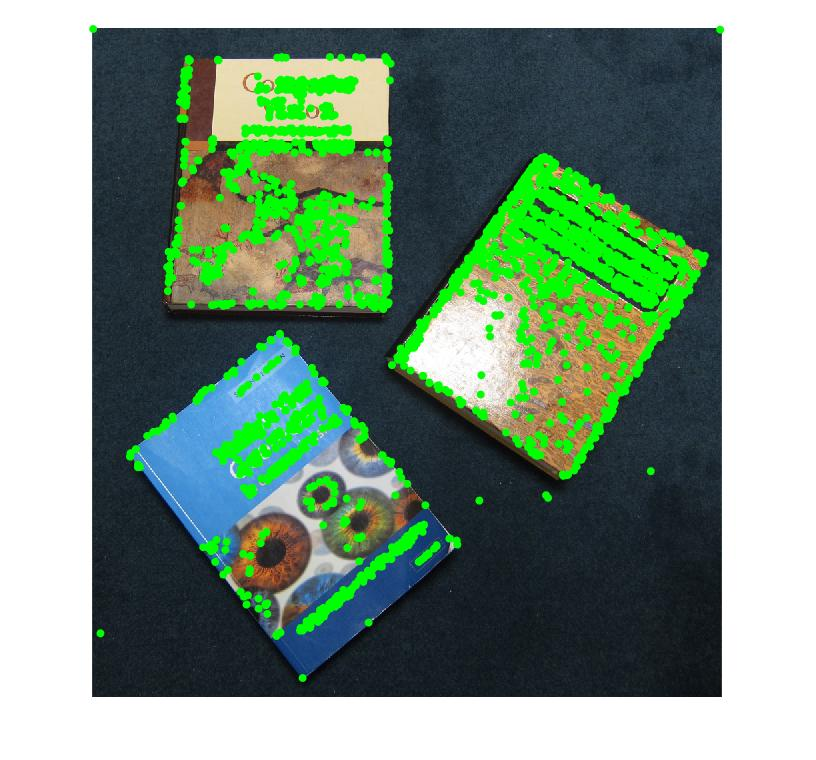
\includegraphics[scale = 0.3]{results/breifPoints1} 
\end{problem}

\newpage
\section{BRIEF Descriptor}

\begin{problem}{2.1}
Code described in makeTestPattern.m and the file testPattern.m has been saved to the file. we choose the method II proposed in the paper for generating the pattern.\\ 
\end{problem}

\begin{problem}{2.2}
Code described in computeBrief.m\\ 
\end{problem}

\begin{problem}{2.3}
Code described in brifLite.m\\ 
\end{problem}



\begin{problem}{2.4}
Code described in testMatch.m. we show the results for the chickenbroth below:\\
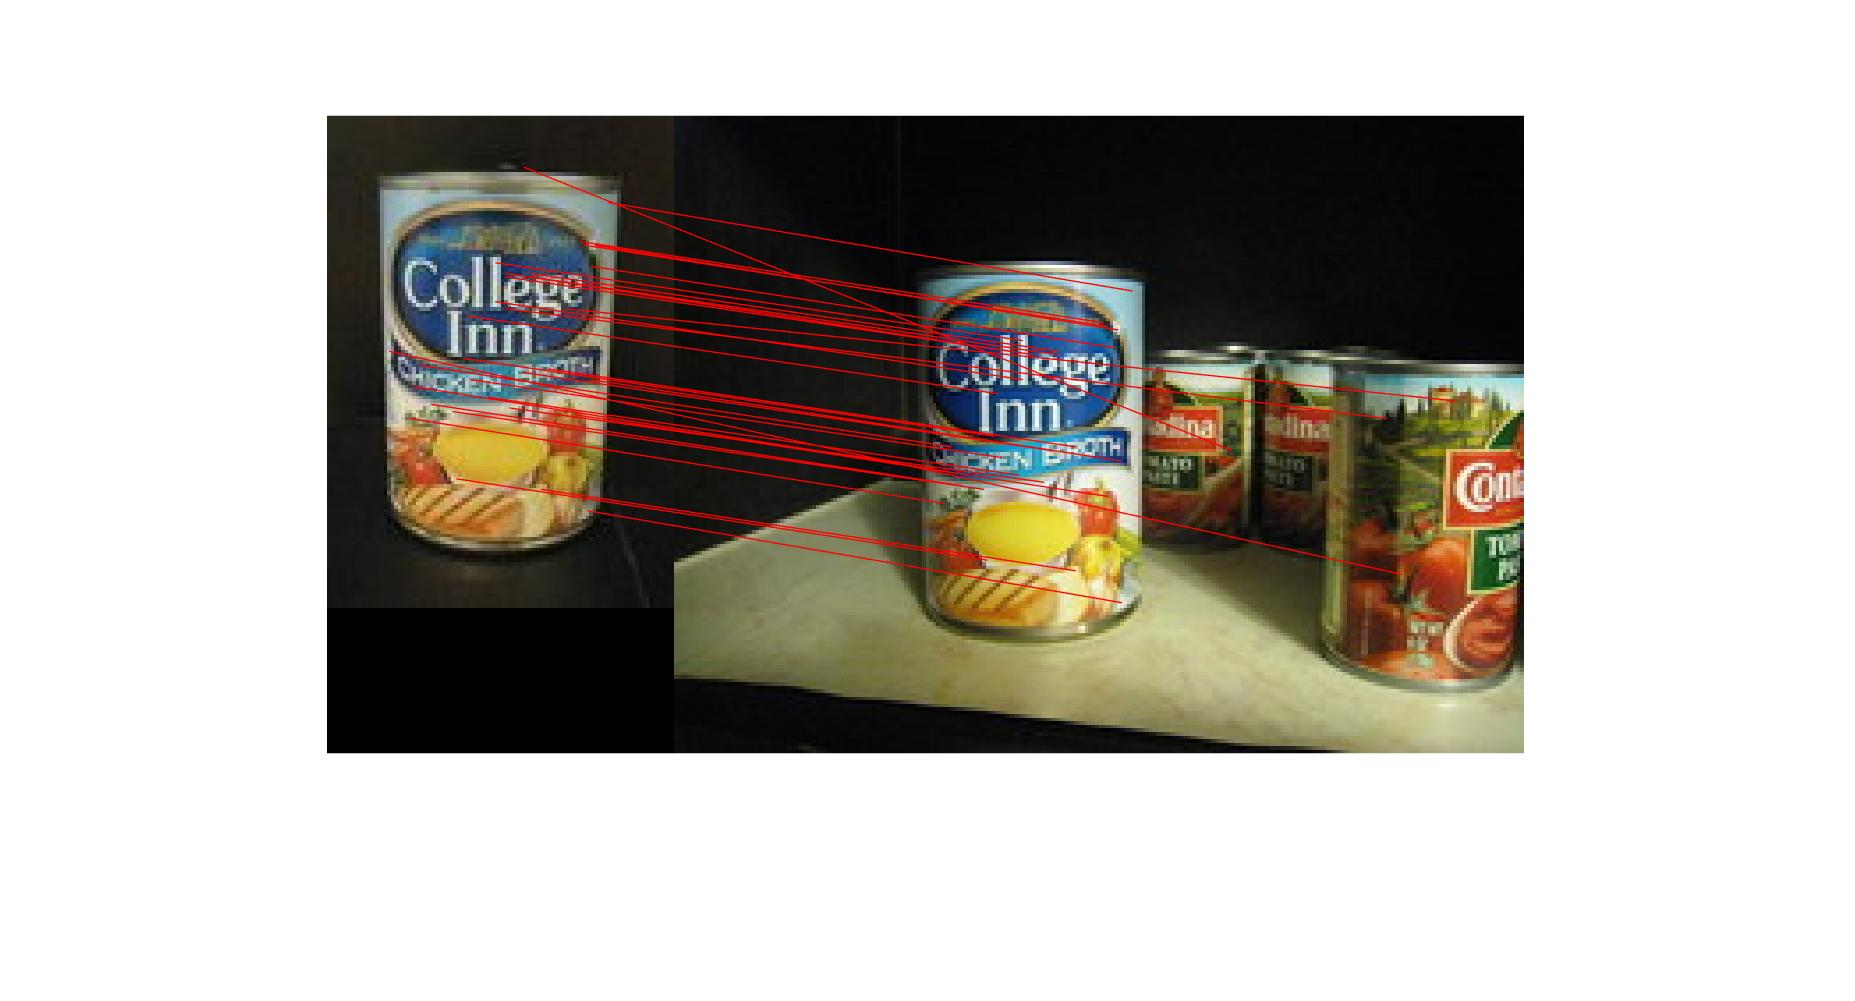
\includegraphics[scale=0.2]{results/matches_plot}\\ 


The results for the incline are shown below:\\
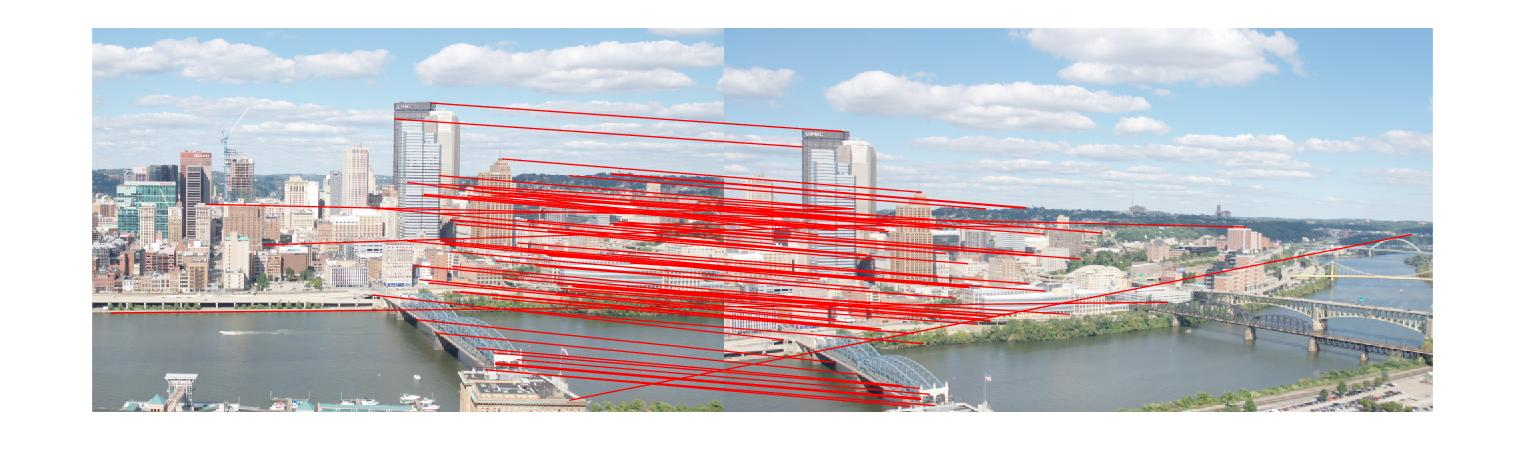
\includegraphics[scale=0.3]{results/incline_match}\\
\newpage
The results for the books dataset is displayed below:\\
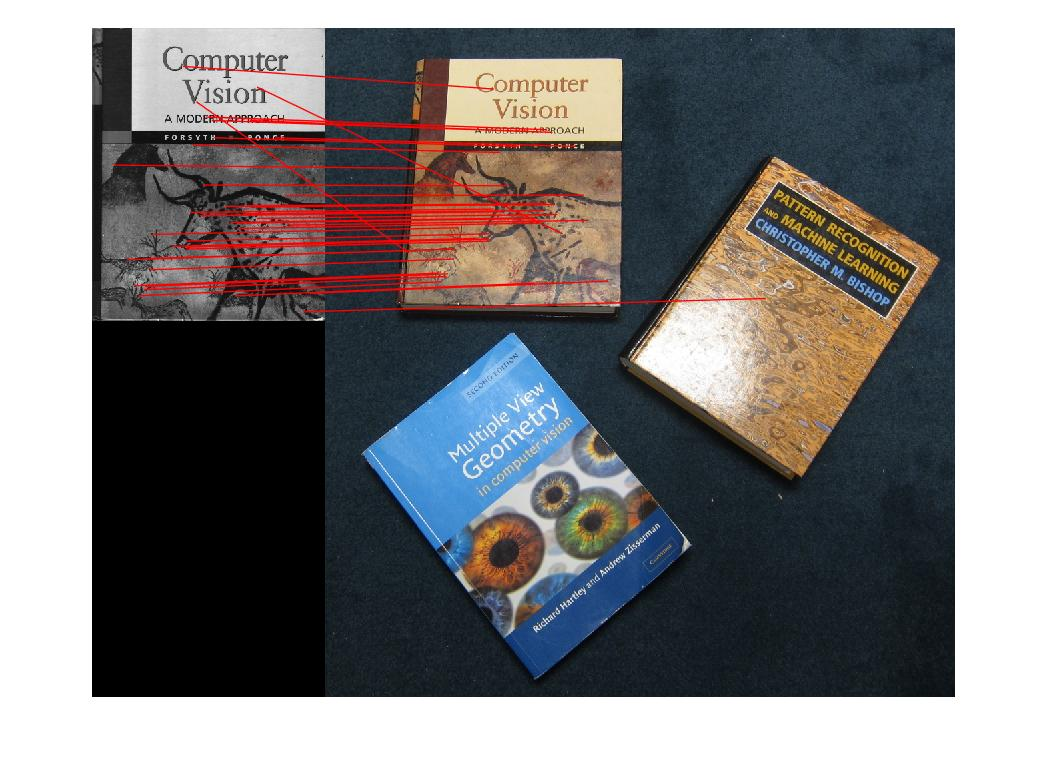
\includegraphics[scale=0.3]{results/books_1}\\
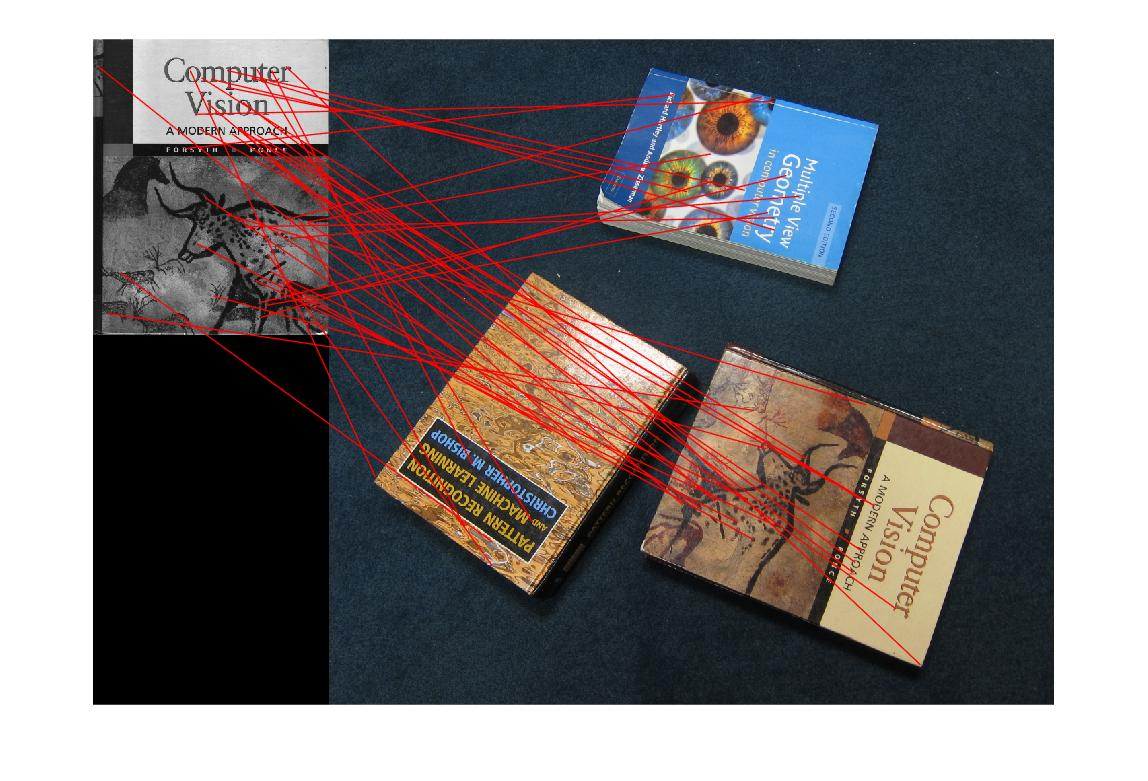
\includegraphics[scale=0.29]{results/books_floor_rot}\\
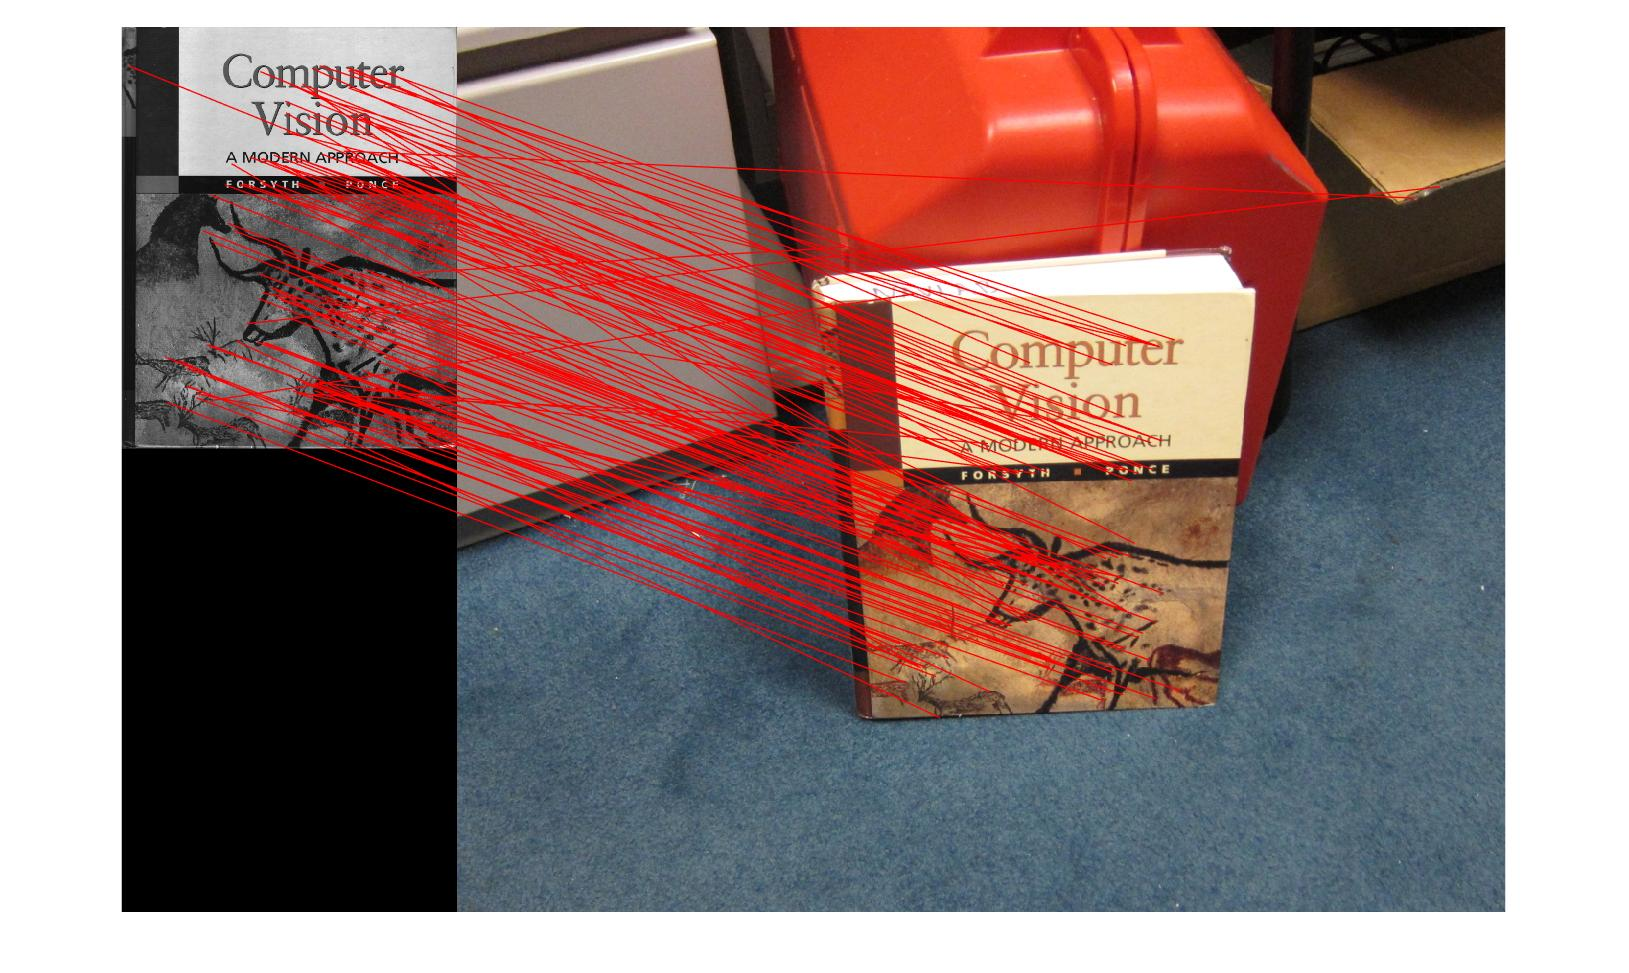
\includegraphics[scale=0.2]{results/books_stand}\\

The results display that the features extracted are not rotation inavariant. The book sample has multiple macthes in the first sample but has less matches in the second rotated image. This is because of scale invariance of the BRIEF discriptor. It can be justified that the discriptor is not rotation invariant as the book in standing position finds multiple matches.
\end{problem}


\begin{problem}{2.5}
The rotation test script is written in briefRotTest.m. The results are shown in the below plot:\\
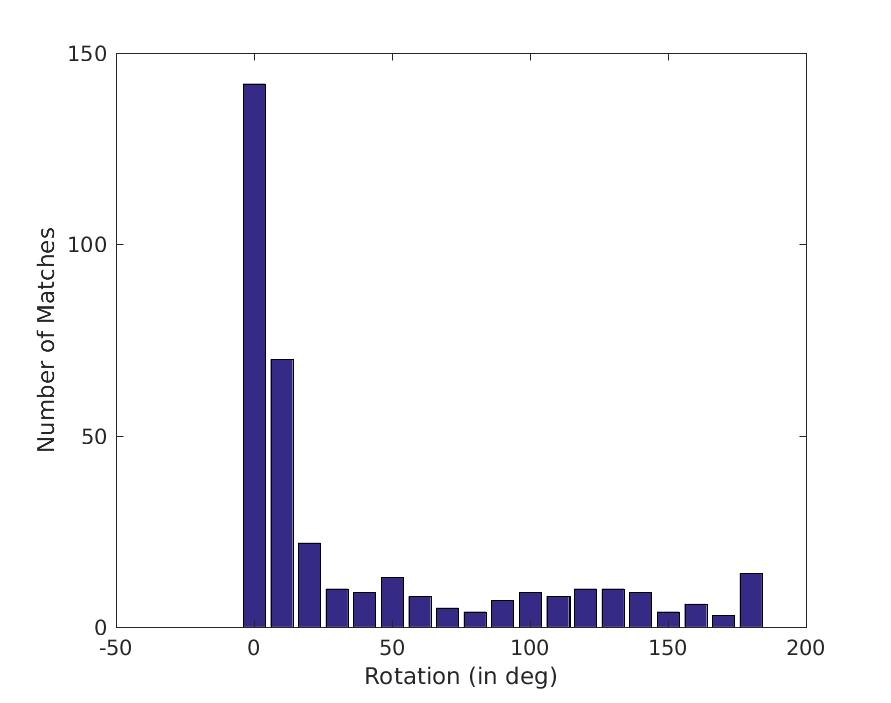
\includegraphics[scale = 0.4]{results/RotTest}

As you can see the descriptor has less error for matches with less rotation and nearly zero matches as it rotates from the original image. This can be attributed to the fact that the BRIEF discriptor is not rotation invariant.
\end{problem}



\section{Planar Homographies}

\begin{problem}{3.1 a)}

let us start by assuming a single point in 3D which projects onto two points  $p = (x_1,y_1,1)$ and $q  = (x_2,y_2,1)$ respectively. The homography H then maps p onto q using an affine transformation and can be written as:
\begin{equation}
\lambda q = H p
\end{equation}

Now lets assume H is a $3x3$ matrix and is given as $H = [H_{11},H_{12},H_{13};H_{21},H_{22},H_{23};H_{31},H_{32},H_{33}]$, then substituting $p = (x_i,y_i,1)$ and $q = (x_2,y_2,1)$ in the above equation gives:

$$\lambda = H_{31}x_1+H_{32}y_1+H_{33}$$
$$\lambda x_2 = H_{11}x_1+H_{12}y_1+H_{13}$$
$$\lambda y_2 = H_{21}x_1+H_{22}y_1+H_{23}$$

By subitituting $\lambda$ we get:

$$(H_{31}x_1+H_{32}y_1+H_{33})x_2 = H_{11}x_1+H_{12}y_1+H_{13}$$
$$(H_{31}x_1+H_{32}y_1+H_{33})y_2 = H_{21}x_1+H_{22}y_1+H_{23}$$

we want to solve for H.  By rearranging the above equations we get,
$$a_{x}^{T}h = 0$$
$$a_{y}^{T}h = 0$$
where \\
$$h = [H_{11},H_{12},H_{13},H_{21},H_{22},H_{23},H
_{31},H_{32},H_{33}^T]$$
$$a_x = (-x_1,-y_1,-1,0,0,0,x_2 x_1, x_2 y_1, x_2)^T$$
$$a_x = (0,0,0,-x_1,-y_1,-1,y_2 x_1, y_2 y_1, y_2)^T$$ 

given a set of corresponding points, we can form the following linear system of equations,
$$Ah = 0$$
\end{problem} 

\begin{problem}{3.1 b)}
The number of elements in h are 9 as it is a 3x3 matrix. 
\end{problem}

\begin{problem}{3.1 c)}
Since H operates on homogeneous coordinates, it is homogeneous itself. We can always divide H by a constant without changing its function.
\[
H = 
 \begin{bmatrix}
  h_{11} & h_{12} & h_{13}\\
  h_{21} & h_{22} & h_{23}\\
  h_{31} & h_{32} & 1\\
 \end{bmatrix}
\]
This matrix is genrated by divding the H matrix by its $H_{33}$. since each point correpondence provides 2 equations, 4 correspondences are sufficient to solve forthe 8 degrees of freedom. 
\end{problem}

\begin{problem}{3.1 d)}
It can be shown that solving $Ah=0$ is equalent to solving the following rayleigh quotient problem(RQP):

\[
min_h \dfrac{h^T (A A^T) h}{h^T h}
\]

the normalization $h^T h$ avoids the selection of the trivial solution $h=0$. The RQP of the above equation is referred to as algebraic least squares and is minimized by choosing h to be the eigenvector corresponding to the smallest eigen value of the eigenvalue problem.
\[
A^T A h = \lambda_{min} h
\]

In the absence of noise, $rank(A^T A) = 8$ and the true homography 
$h \in null(A^T A)$.
\end{problem}

\section{Planar Homographies:Implementation}
\begin{problem}{4.1}
Code has been written to computeH.m
\end{problem}

\section{RANSAC}
\begin{problem}{5.1}
Code has been written to ransacH.m
\end{problem}

\newpage

\section{Stitching it together:Panaromas}
\begin{problem}{6.1}
The code has been updated to imageStitching.m\\ The results using homography computation are saved :
 
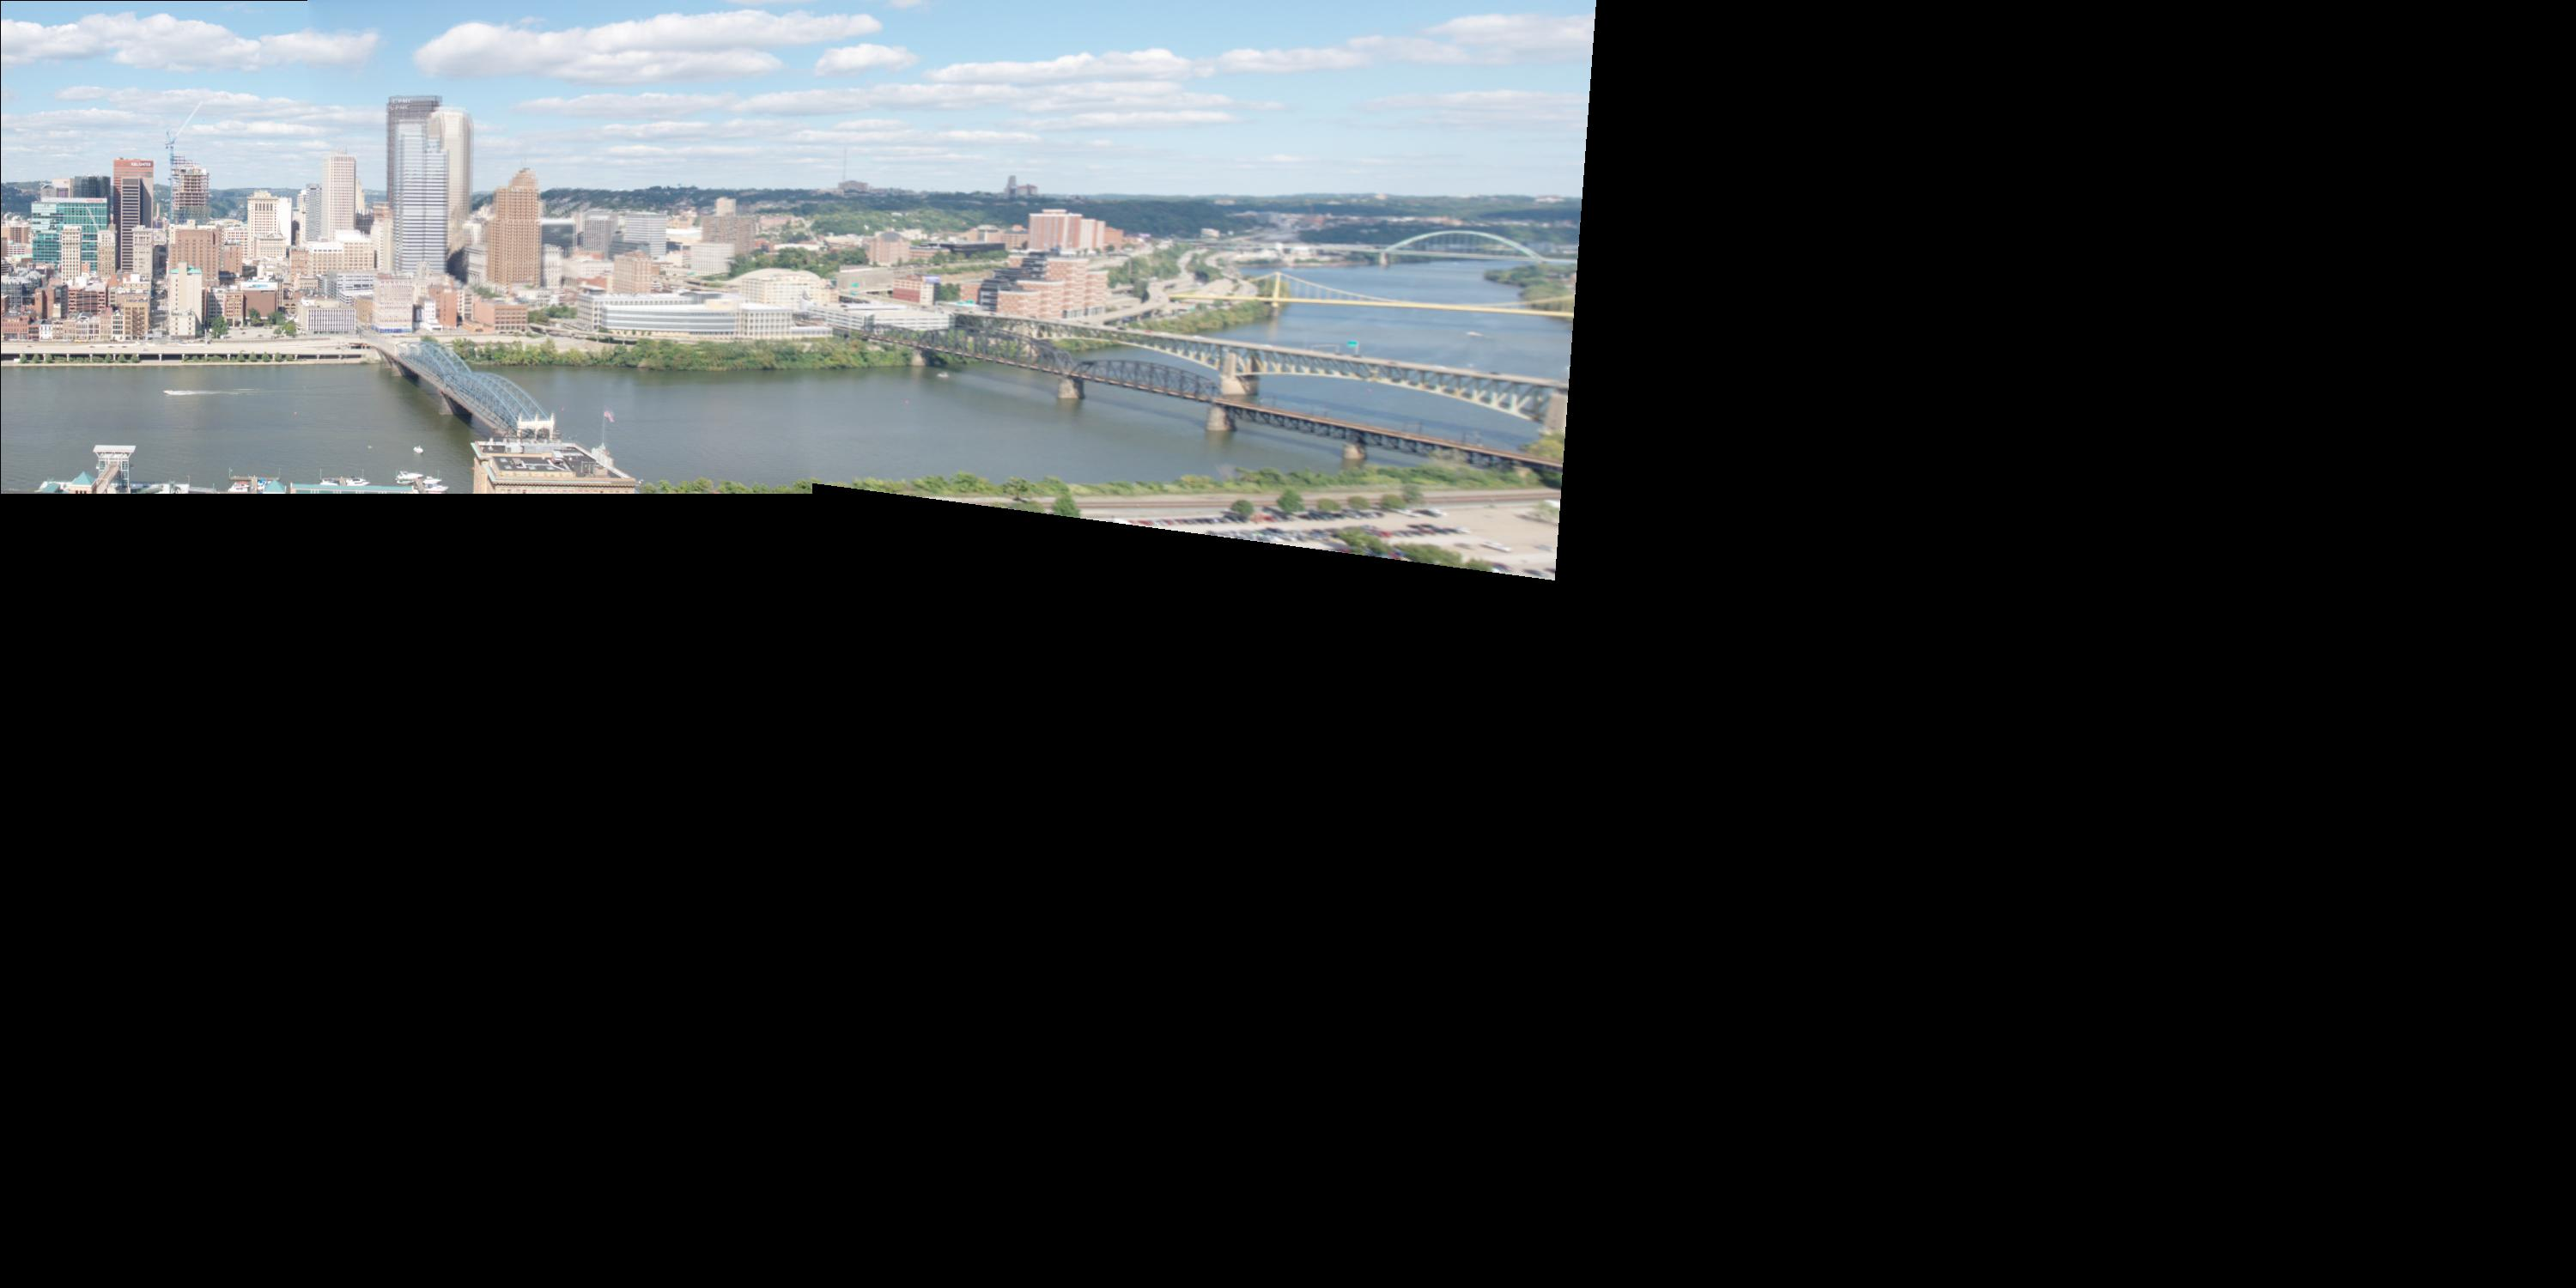
\includegraphics[scale=0.1]{results/q6_1}

The image are scaled to 3000 1500 for all the following panaroma tests to help understand the exact homography warping.
\end{problem}

\begin{problem}{6.2}
The code has been updated to $imageStitching_noClip.m$ \\

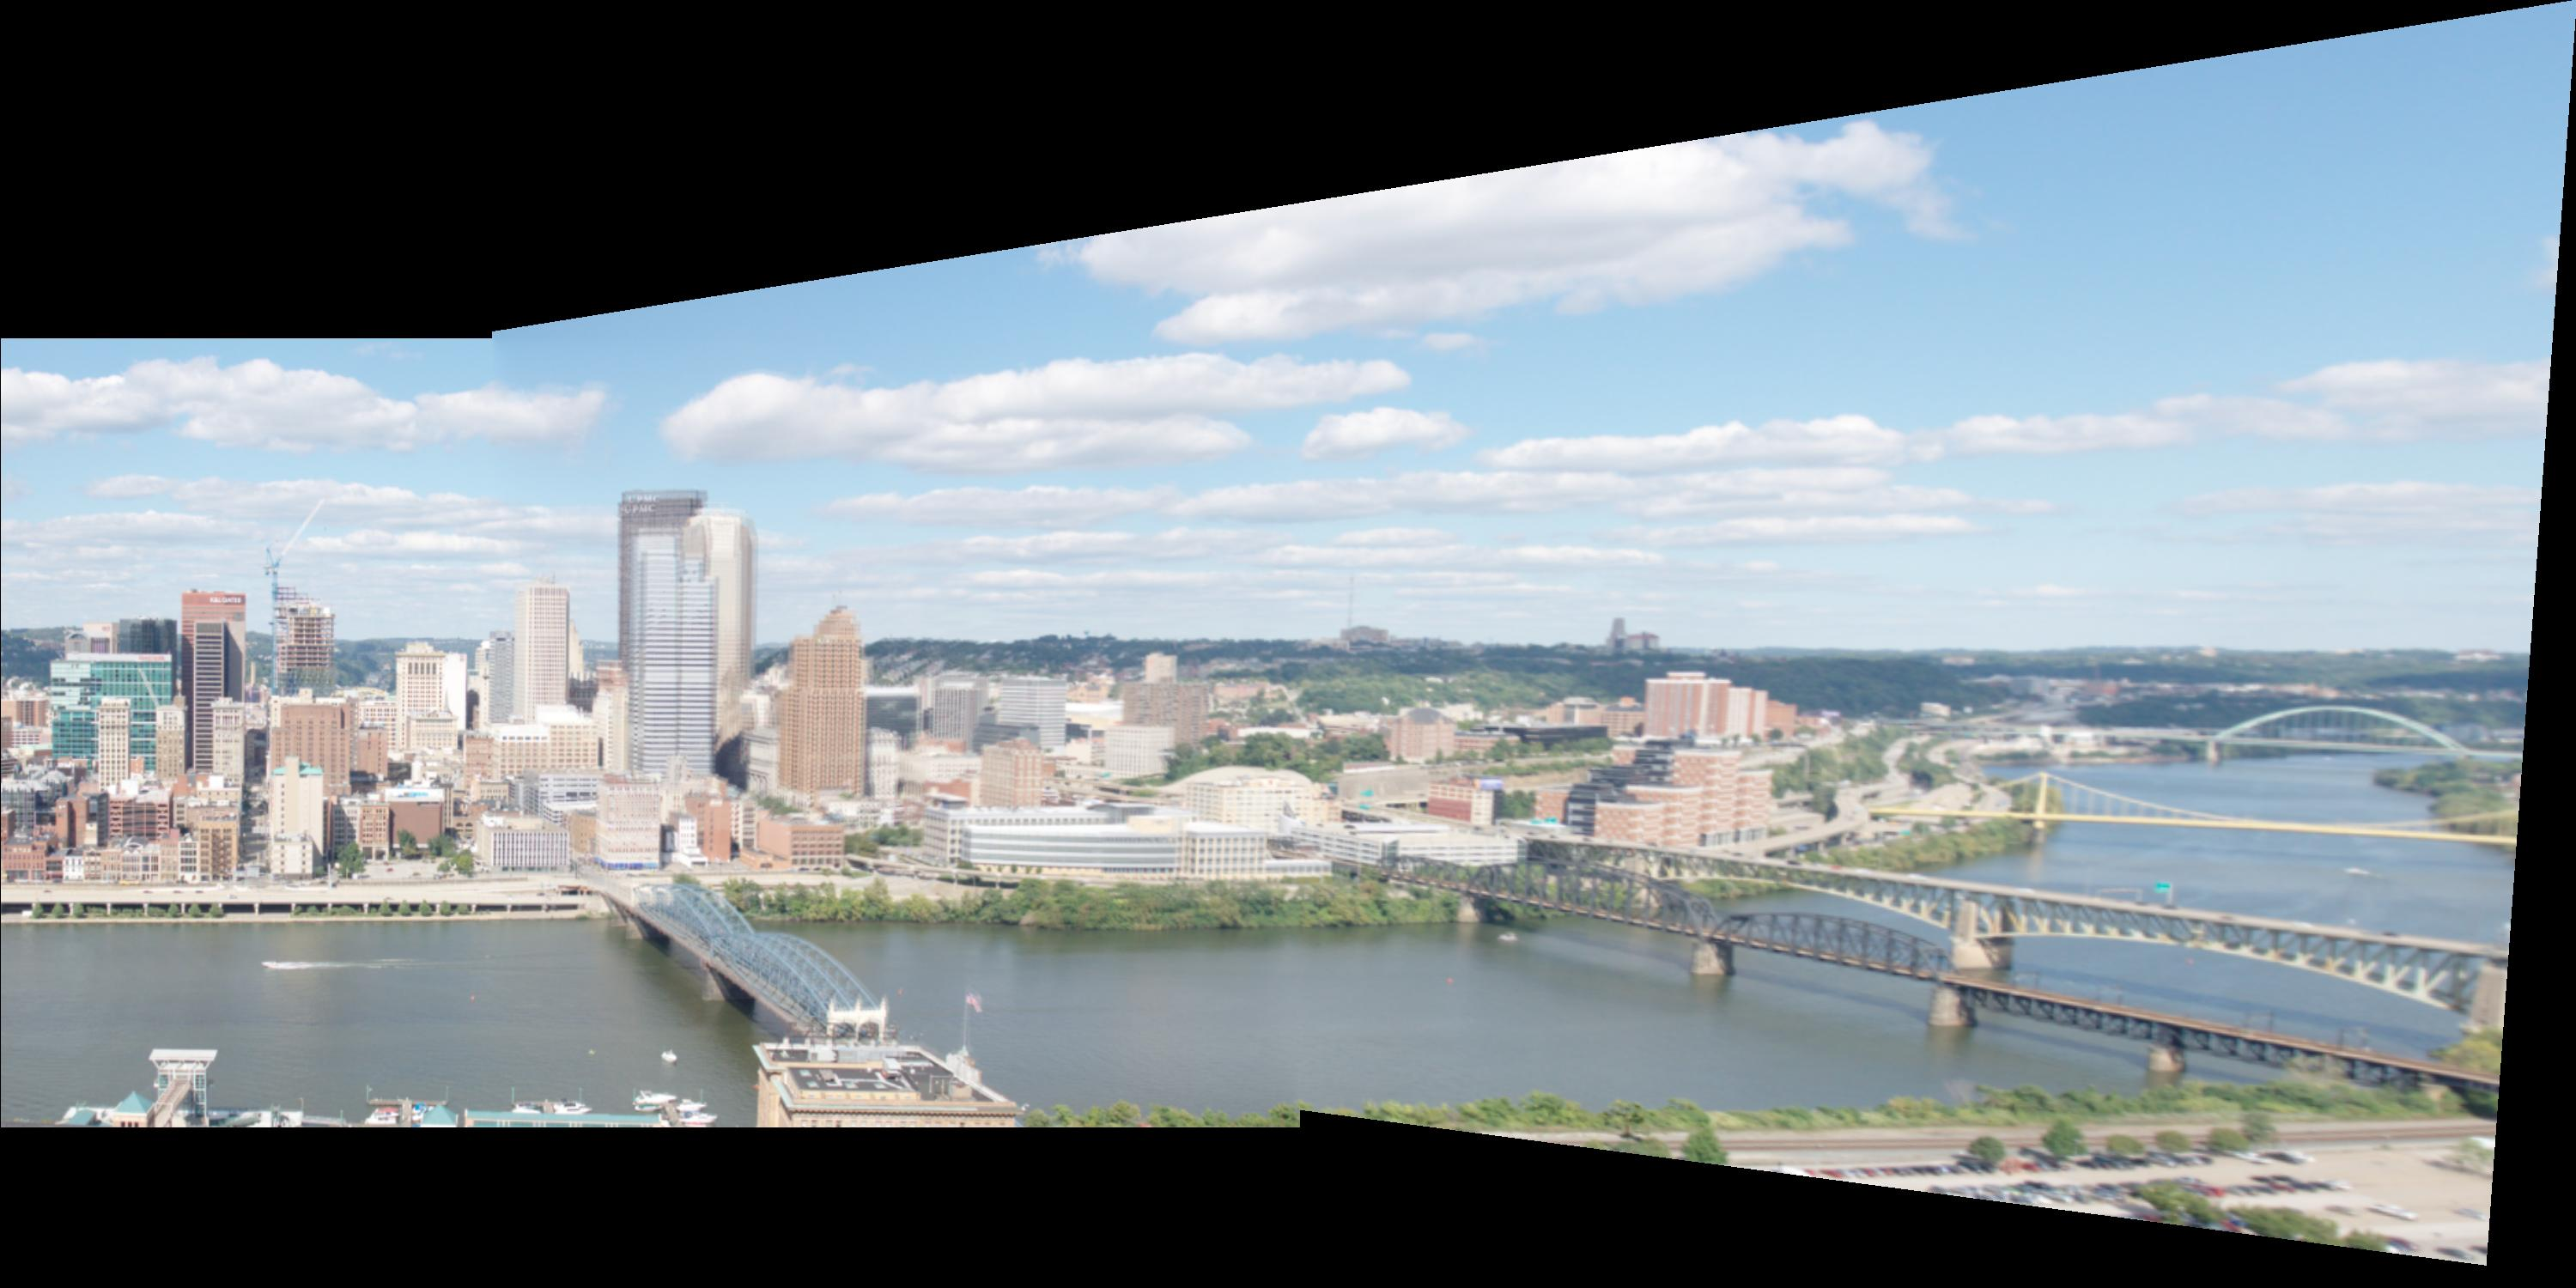
\includegraphics[scale=0.1]{results/q6_2_pan}\\
\end{problem}

\begin{problem}{6.3}
The code has been updated to $imageStitching_noClip.h$ \\
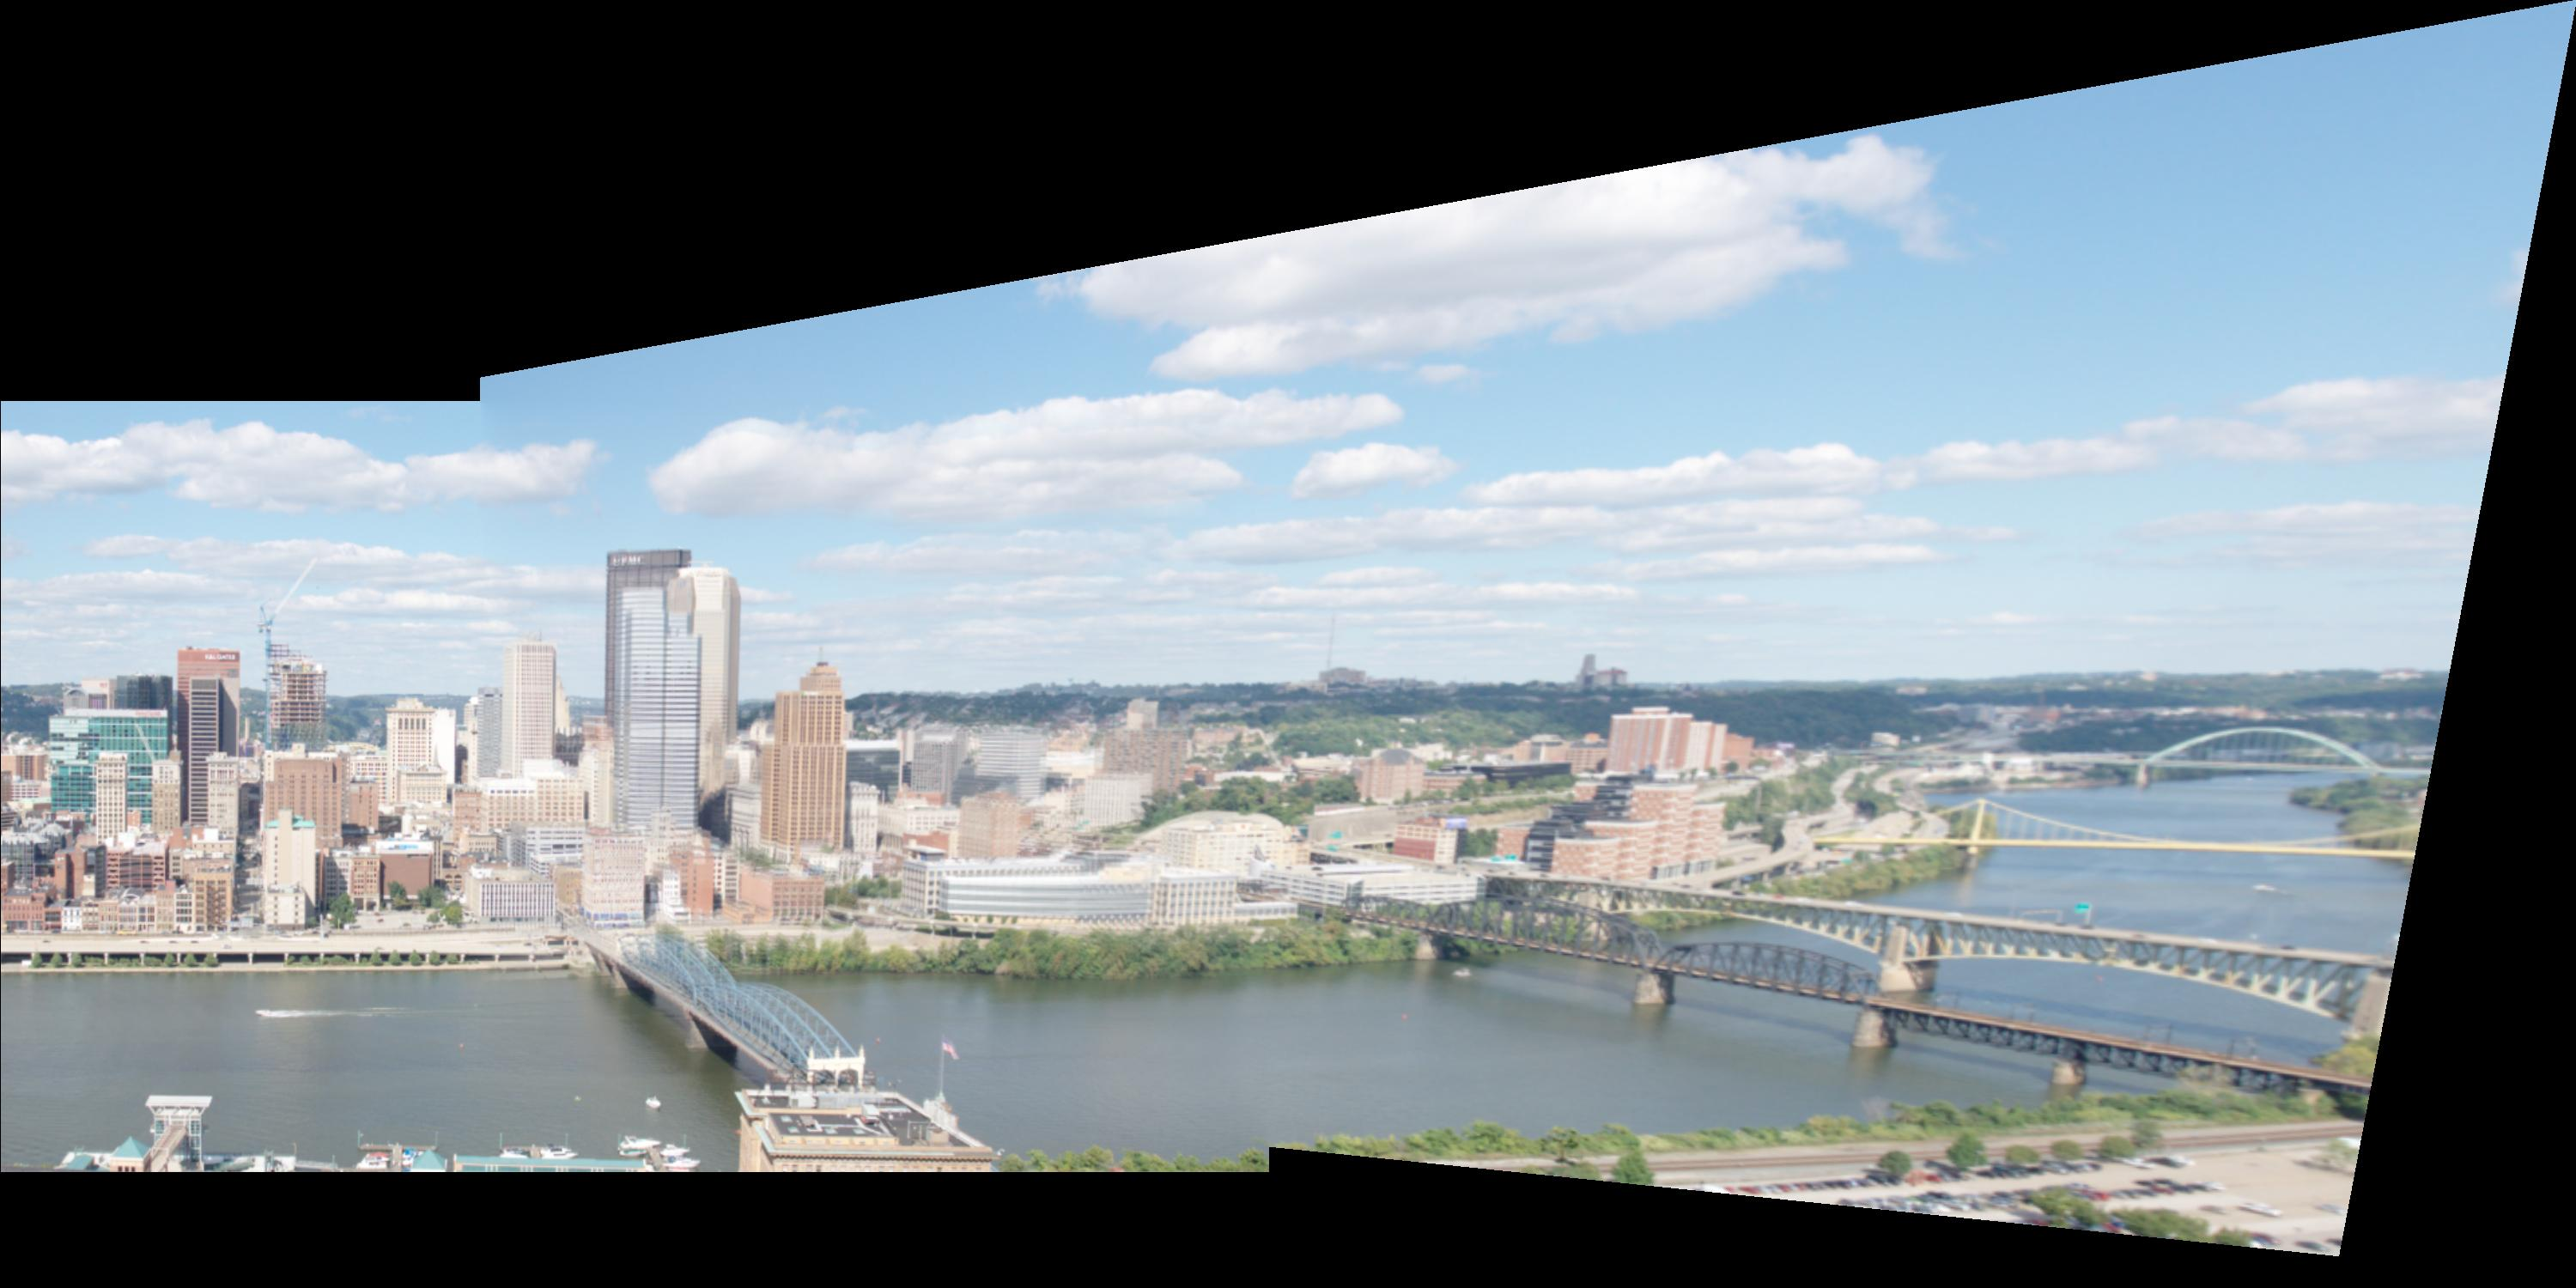
\includegraphics[scale=0.1]{results/q6_3}\\
\end{problem}
\newpage

\section{extra credit}

For all the experiments below we use the rotation variation from 0 to 180 degrees at the step of 10 degrees. And the scale is from 0.2 to 4 times of the image size with a step of 0.3

\begin{problem}{7.1}
From the rotation test in question 2.5. You can see that the BRIEF discrptor doesnt perform well for the dataset with varied rotation. In order to improve the accuracy of matching we propose a rotation invariant BRIEF descriptor. We compute the gradient magnitude and orientation using pixel difference. An orientation histogram is formed from the gradient orientations of sample points within a region around the keypoint. The orientation histogram has 36 bins covering the 360 degrees range of orientation. The peaks in the orientation histogram represent the dominent direction of local gradients. we rotate the image patch with the dominent direction and compute the BRIEF discriptor on the rotated patch. We show the results of the matching with rotation and translation below:\\


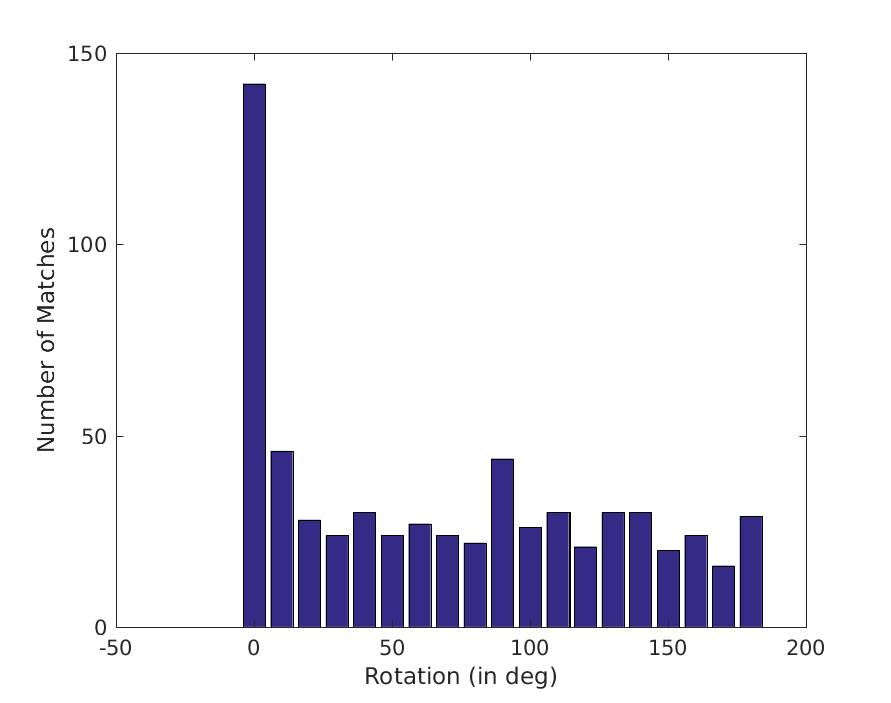
\includegraphics[scale=0.2]{results/EC1_RotErr}
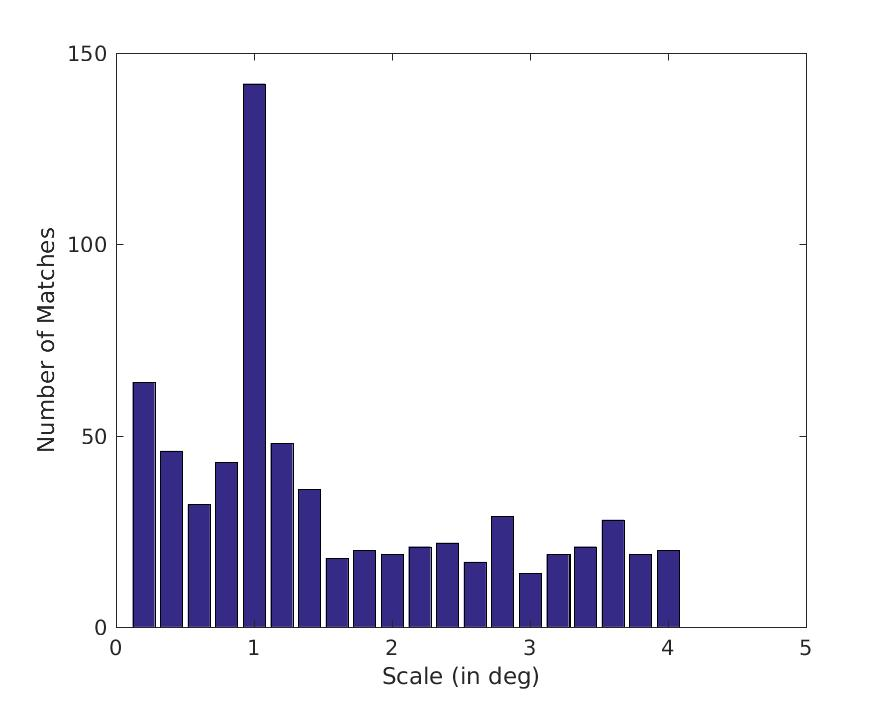
\includegraphics[scale=0.2]{results/EC1_ScalErr}
\end{problem}

\begin{problem}{7.2}
When the matching is done between different scales of the same image. the matches reduced by a significant amount. We solve this problem by taking scale invariant features while computation of the BRIEF discriptor. This is computed by finding the scale which best describes the key point and computing the brief descriptor at the patch scale. This shows a tremendous improvement in the accuracy of matches for both the rotation and the scale tests. Both the codes have been excecuted in $computeBrief_rotate.m$\\


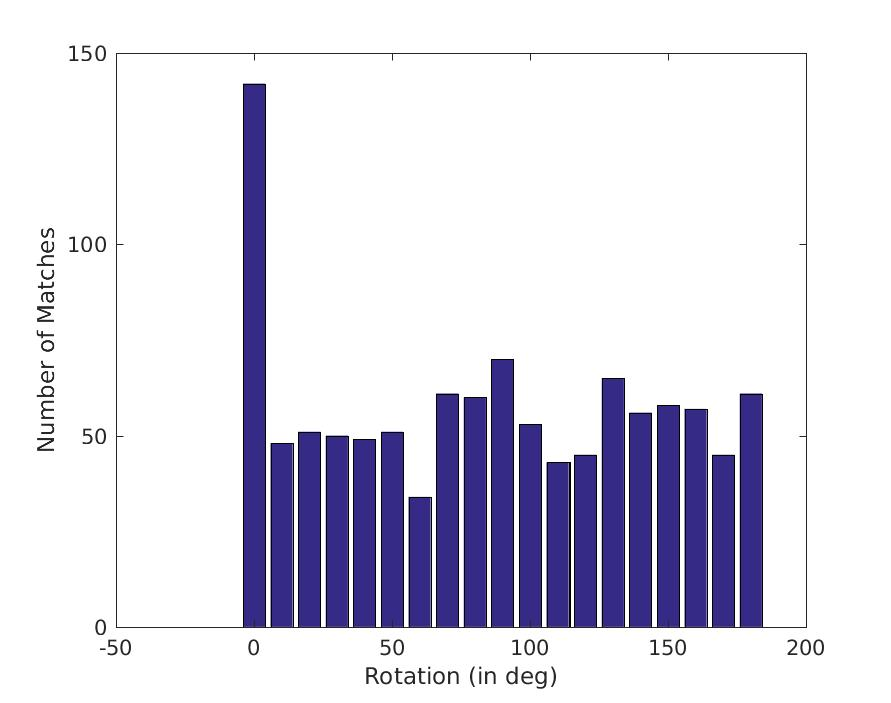
\includegraphics[scale=0.2]{results/EC2_RotErr}
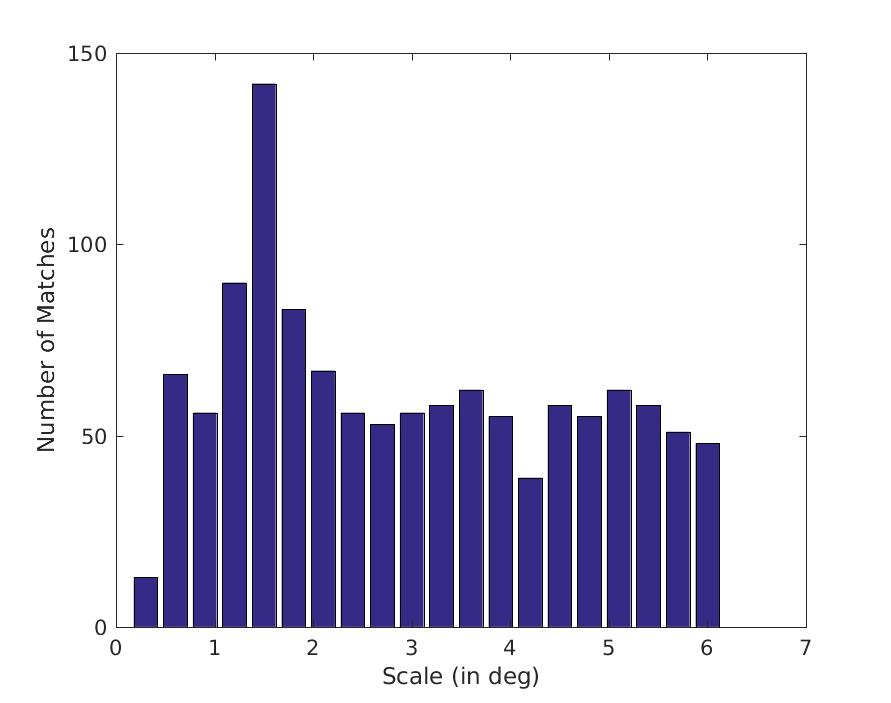
\includegraphics[scale=0.2]{results/EC2_ScalErr}
\end{problem}
\end{document}